\section{Data selection}
\label{sec:dataselection}

\begin{table}[t]
\centering
\begin{tabular}{ | l| l|  }
\hline
Healpix order & 6, 7  \\ 
Weeks & $9-745$  \\ 
Emin & 1 GeV \\
Emax & 10 GeV \\
Instrument Response Functions (IRFs) & \verb|P8R3_SOURCEVETO_V3| \\
EVCLASS & 2048 (Source Veto)  \\ 
EVTYPE & 1 (Front)  \\
ZMAX & 90 \\
\hline
\end{tabular}
\caption{Fermi Tools settings used for the 14-year data set analysis. }
\label{tab:settings}
\end{table}

We process the \fermi data through the Fermi Tools suite \cite{Fermitools} to produce a full-sky map of photon counts for gamma-ray energies in the (1-10) GeV  range. We choose this range as a suitable balance between high statistics (which occurs at lower energies) and good angular resolution (which is better the higher the energy) of the detector, as well as being able to confront our results with those of Ref. \cite{Cuoco-1pdf}.

We consider the first 14 years of data collected by the \fermi (specifically, from week 9 to week 745 of operation), and Pass 8 event selection \cite{Fermi-LAT:2013jgq,Bruel:2018lac}. We adopt the \verb|P8R3_SOURCEVETO_V3| instrument response functions (IRFs), event class (EVCLASS) 2048 ({\tt SOURCEVETO}) and event type (EVTYPE) 1 (\verb|FRONT|). We used standard quality selection criteria, i.e. \verb|DATA QUAL==1| and
\verb|LAT CONFIG==1|.
The atmospheric gamma rays from the Earth limb emission is removed by adopting a cut
on the maximum zenith angle ZMAX of 90 degrees.
\verb|FRONT| events refer to gamma-rays detected by the first layers of the tracking module of the \fermi detector, and are optimised in order to have a better angular resolution, which is a crucial requirement for our analysis. 
The {\tt SOURCEVETO} class of events achieves good suppression of the charged cosmic-ray (CR) background while still retaining a large event statistics. All those settings are summarised in Table \ref{tab:settings}. Finally, the maps are constructed with equal-area pixels by adopting the Healpix \cite{healpix} pixelisation scheme of order $n=6$ ($N_{\rm side} = 64$ resolution, which corresponds to $0.92^\circ$ pixel side) although for testing we will also use maps with order $n=7$ ($N_{\rm side} = 128$).  
The photon count map, in counts per pixel, for the 14 year data set is shown in Fig. \ref{fig:FermiMap}. This is the map to which we will apply the CNN to extract the source-count distribution of gamma-ray sources. 

\begin{figure}[t]
\centering
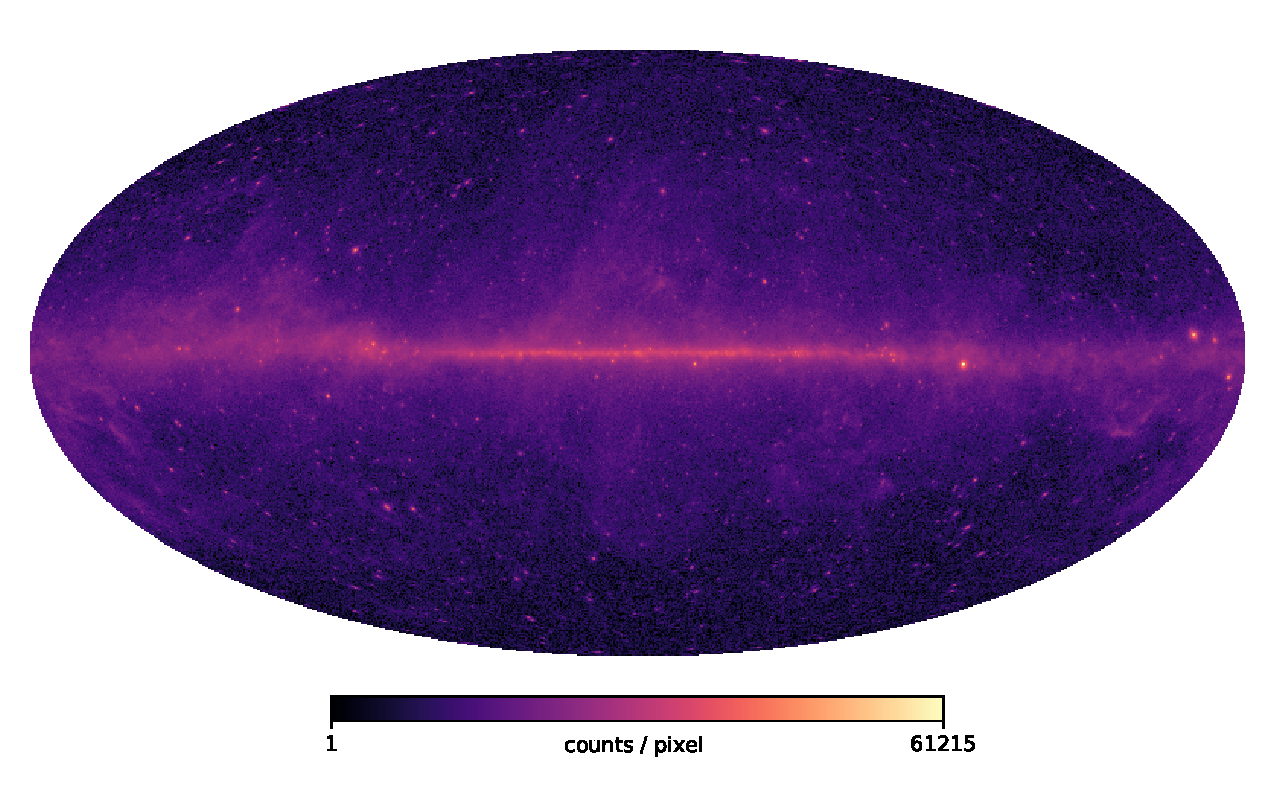
\includegraphics[scale=0.6]{img/data_selection/mappa_fermi.pdf}
\caption{\fermi photon-counts map in units of counts per pixel in the 1-10 GeV energy range}  for the 14-years dataset,  at the Healpix resolution $N_{\rm side} = 128$ ($n=7$). 
\label{fig:FermiMap}
\end{figure}



Using the \fermi tools we further extract
the \fermi exposure map and the point-spread-function (PSF) for photon energies in $(1,10)$ GeV, which will be needed to construct the synthetic maps used to train and validate the CNN.
Some care is required, since the PSF is a rapidly varying function of energy.
Following previous works \cite{Cuoco-1pdf,Fornasa:2016ohl},
we build the $(1,10)$ GeV mean PSF by averaging the energy-dependent PSF in the $(1,10)$ GeV energy range with a $E^{-2.4}$ weight, corresponding to the approximate energy spectrum of the high Galactic latitude gamma-ray sky. The average exposure map in the $(1,10)$ GeV energy bin and the averaged PSF profile are shown in Fig. \ref{fig:exposure}  and in Fig. \ref{fig:PSF}, respectively. The \fermi exposure slightly changes with energy, although its variation inside our energy bin is small.

A further dataset we will use is the catalog of resolved sources.
In particular, we will employ the recently released  Data Release 3 of the fourth \fermi catalog of gamma-rays sources (4FGL-DR3) \cite{2022ApJS..260...53A}, which increments the previous release to 12 years of data taking and contains 6658 resolved sources. From this catalog, we obtain the (1-10) GeV source-count distribution in the resolved regime, shown in Fig. \ref{fig:dNdS-annotato}. 
The detailed procedure with which we obtain the $\dnds$ from the list of sources is described in Appendix B of \cite{Cuoco-1pdf}.
Here and through the rest of the manuscript $S$ will always refer to an integral flux in the range 1-10 GeV.
The blue points refer to the regime in which the catalog is fully efficient in detecting sources, while the gray points denote sources for which the \fermi sensitivity to point sources starts degrading. 
Our aim is to infer the behaviour of the source count in the unresolved regime, i.e., for source fluxes below $S_{\rm th} \sim 2 \cdot 10^{-10}$ cm$^{-2}$ s$^{-1}$ by adopting a CNN technique.
We stress that in the following the $\dnds$ of resolved sources will be used only for comparison with the result of the CNN analysis, which are completely independent from it.
Thus, the fact that we use 14 years of data while the catalog is based on 12 years does not have an impact on the analysis.

\begin{figure}[t]
\centering
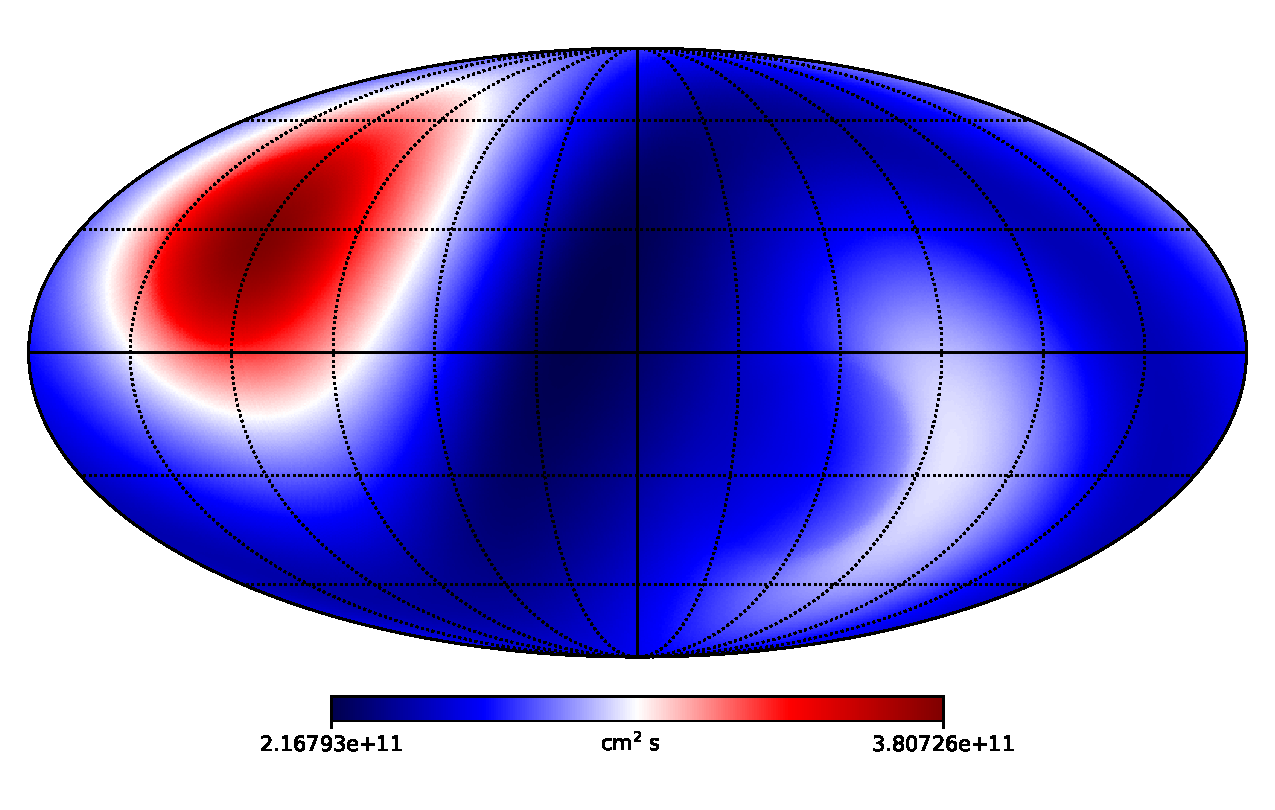
\includegraphics[scale=0.6]{img/data_selection/exposure.pdf}
\caption{\fermi mean exposure map in the 1-10 GeV energy range for the 14-years data set, in units of cm$^2$ s,  at the Healpix resolution $N_{\rm side} = 128$ ($n=7$).} 
\label{fig:exposure}
\end{figure}

\begin{figure}[t]
\centering
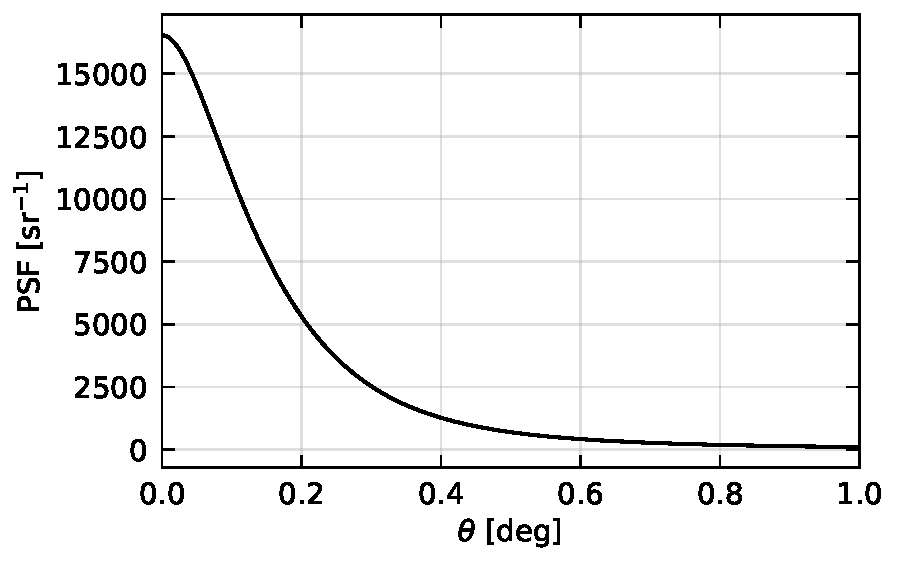
\includegraphics[scale=0.6]{img/data_selection/PSF.pdf}
\caption{Average \fermi point spread function (PSF) for energies in $(1, 10)$ GeV.}
\label{fig:PSF}
\end{figure}

%---------------------------------

